% !Mode:: "TeX:UTF-8"
%!TEX program  = xelatex

%\documentclass{cumcmthesis}
\documentclass[withoutpreface,bwprint]{cumcmthesis} %去掉封面与编号页

\usepackage{url}
\title{论文标题}
\tihao{A}
\baominghao{4321}
\schoolname{东南大学}
\membera{卢立强}
\memberb{喻泽弘}
\memberc{杜昕昱}
\supervisor{老师}
\yearinput{2019}
\monthinput{05}
\dayinput{11}

\begin{document}

 \maketitle
 \begin{abstract}

这里是摘要

\keywords{\quad  曲线拟合\quad   非线性优化模型\quad  受力分析}
\end{abstract}

%目录
\tableofcontents

\section{问题重述与提出}

\subsection{问题的重述}

随着我国科技发展,现代物流观念对个行业发展都产生了重要影响,RGV(有轨穿梭小车)的产生促进了自动化系统和仓库的发展,它可用于各类高密度储存方式的仓库,小车通道可设计任意长,安全性更高,有效地提高效率。RGV小车可以十分方便地与其他物流系统实现自动连接,按照计划进行物料的输送,而其中对于小车的动态调度策略的设计将会影响整个系统的效率。

RGV小车根据指令能自动控制移动方向和距离,并自带一个机械手臂、两只机械手爪和物料清洗槽,能够完成上下料及清洗物料等作业任务,RGV同一时间只能执行移动、停止等待、上下料和清洗作业中的一项。我们的目标就是要设计智能RGV的动态调度策略,使得系统的作业效率最大化。


\subsection{问题的提出}

针对三种情况:

(1)一道工序的物料加工作业情况,每台CNC安装同样的刀具,物料可以在任一台CNC上加工完成;

(2)两道工序的物料加工作业情况,每个物料的第一和第二道工序分别由两台不同的CNC依次加工完成;

(3)CNC在加工过程中可能发生故障(据统计:故障的发生概率约为1\%)的情况,每次故障排除(人工处理,未完成的物料报废)时间介于10~20分钟之间,故障排除后即刻加入作业序列。要求分别考虑一道工序和两道工序的物料加工作业情况。

我们完成如下两个任务:

任务1:对一般问题进行研究,给出RGV动态调度模型和相应的求解算法;

任务2:利用表1中系统作业参数的3组数据分别检验模型的实用性和算法的有效性,给出RGV的调度策略和系统的作业效率,并将具体的结果分别填入附件2的EXCEL表中。

\section{问题分析}

\subsection{问题的分析}

\textbf{针对任务一:}

任务一分析

\textbf{针对任务二:}

任务二分析

\section{模型的假设}


\subsection{模型的假设}

\begin{itemize}
\item 假设一
\item 假设二
\item 假设三
\item 假设四
\end{itemize}

\section{符号说明}
\begin{center}
\begin{table}[!htbp]
\centering
\caption{这是一张三线表}\label{tab:aStrangeTable}\centering%添加标题 设置标签
\begin{tabular}{c|c|c}\hline
符号& 表示含义& 单位\\\hline
Steve Jobs& 001& Male\\
Bill Gates& 002& Female\\\hline
\end{tabular}
%\caption{这是一张三线表}\label{tab:aStrangeTable}  标题放在这里也是可以的
\end{table}
\end{center}

\begin{table}[!htbp]
\caption{标准三线表格}\label{tab001} \centering
\begin{tabular}{ccccc}
\toprule[1.5pt]
$D$(in) & $P_u$(lbs) & $u_u$(in) & $\beta$ & $G_f$(psi.in)\\
\midrule[1pt]
 5 & 269.8 & 0.000674 & 1.79 & 0.04089\\
10 & 421.0 & 0.001035 & 3.59 & 0.04089\\
20 & 640.2 & 0.001565 & 7.18 & 0.04089\\
\bottomrule[1.5pt]
\end{tabular}
\end{table}

\section{模型建立与求解}

blablabla。。。

插入图片:
\begin{figure}[!h]
\centering
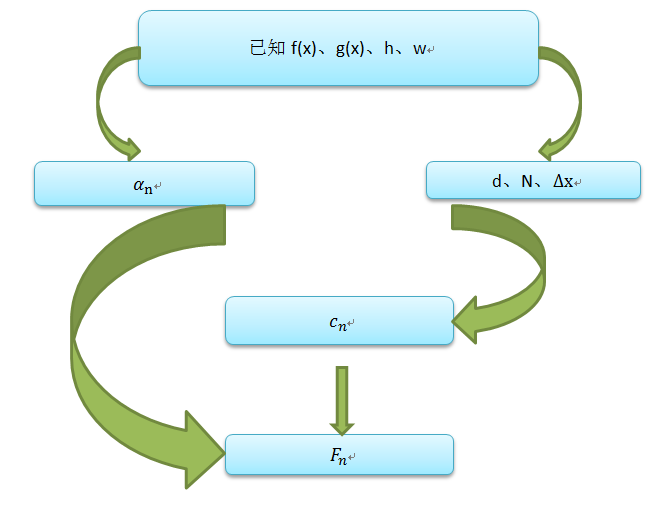
\includegraphics[width=.6\textwidth]{1.png}
\caption{任务流程图}
\end{figure}
\subsection{任务一模型的情况}
\subsubsection{任务一模型的建立}
分条列举:
\begin{itemize}
\item[(1)] 
第一条
\begin{equation}
X(k)=\sum_{n=0}^{N-1} x(n)e^{-j \frac{2 \pi}{N} k n}=\sum_{n=0}^{N-1} x(n) W_N^{kn},\quad k=0,1,...,N-1.
\end{equation}

\item[(2)]
第二条
\begin{equation}
X_i=X_{i-1}+x
\end{equation}
\item[(3)]
第三条
$$ f(x)=\left\{
\begin{aligned}
x & = & \cos(t) \\
y & = & \sin(t) \\
z & = & \frac xy
\end{aligned}
\right.
$$
\item[(4)]
第四条
\end{itemize}
\subsubsection{任务一模型的求解}
这里我们可以插入流程图
\subsection{任务二模型的情况}
\subsubsection{任务二模型的建立}
\subsection{任务二模型的求解}

\section{模型的评价}
\subsection{模型的优点}
\subsection{模型的缺点}
\subsection{模型的改进}
\subsection{模型的推广与应用}
%参考文献
\begin{thebibliography}{9}%宽度9
 \bibitem{bib:one} 大学物理
 \bibitem{bib:two} 高等数学
\end{thebibliography}

\newpage
%附录
\begin{appendices}
\section{遗传算法--python 源程序}
\begin{lstlisting}[language=python]
print helloworld!
 \end{lstlisting}
 \section{程序--X代码}
\begin{lstlisting}[language=c]
cout<<"helloworld";
 \end{lstlisting}
\end{appendices}

\end{document} 